\chapter{Detail design}\label{ch:detail_design}
%**********************************************


In this section, you need to capture your design, which should include the following: 
\begin{itemize}
  \item Design rationale, i.e. what your thinking was behind the design.
  \item References to literature/sources as appropriate \cite{WebsiteOpAmp}, but preferably in the intro above.
  \item You can assume the reader is in their third year of their E\&E engineering degree, and that they will not need detailed explanations of trivial information (e.g. what a resistor is, or what Ohm's law is).  
  \item Design calculations, for example to determine resistor values and capacitor values, or to check for allowed voltage and current ranges and levels. These calculations should also give expected outputs, which hopefully matches the simulated values. 
  \item Analysis of given or expected input conditions. 
  \item Expected values and ranges based on your design. 
  \item Explain your choice of supply by referring to the advantages and disadvantages of each. 
  \item Circuit diagram like the one in Figure \ref{fig:circuit_diagram}. I used ``print to PDF'' from LTSpice,  but feel free to use a cropped screengrab if you are PDF-challenged and do not have a PDF printer (there are some free PDF creators online). Also have a look at the demo video on SUNLearn. 
\end{itemize}

\noindent For your benefit, here is how to write values with units: \SI{150}{\milli\ohm} or \SI{199}{myUnits}, and this is how we write ranges: from \SI{2} to \SI{5}{\kilo\volt}.\\

\noindent Here is an inline equation $ \frac{55}{45+3}$.\\Here is a numbered equation in Eq. \ref{eq:myNumberedEquation}.
\begin{equation}
   a = \frac{55}{45+3}
   \label{eq:myNumberedEquation}. 
\end{equation}. 

\begin{figure}[H]
 \footnotesize
   \centering
   \begin{subfigure}[]{0.45\textwidth}
        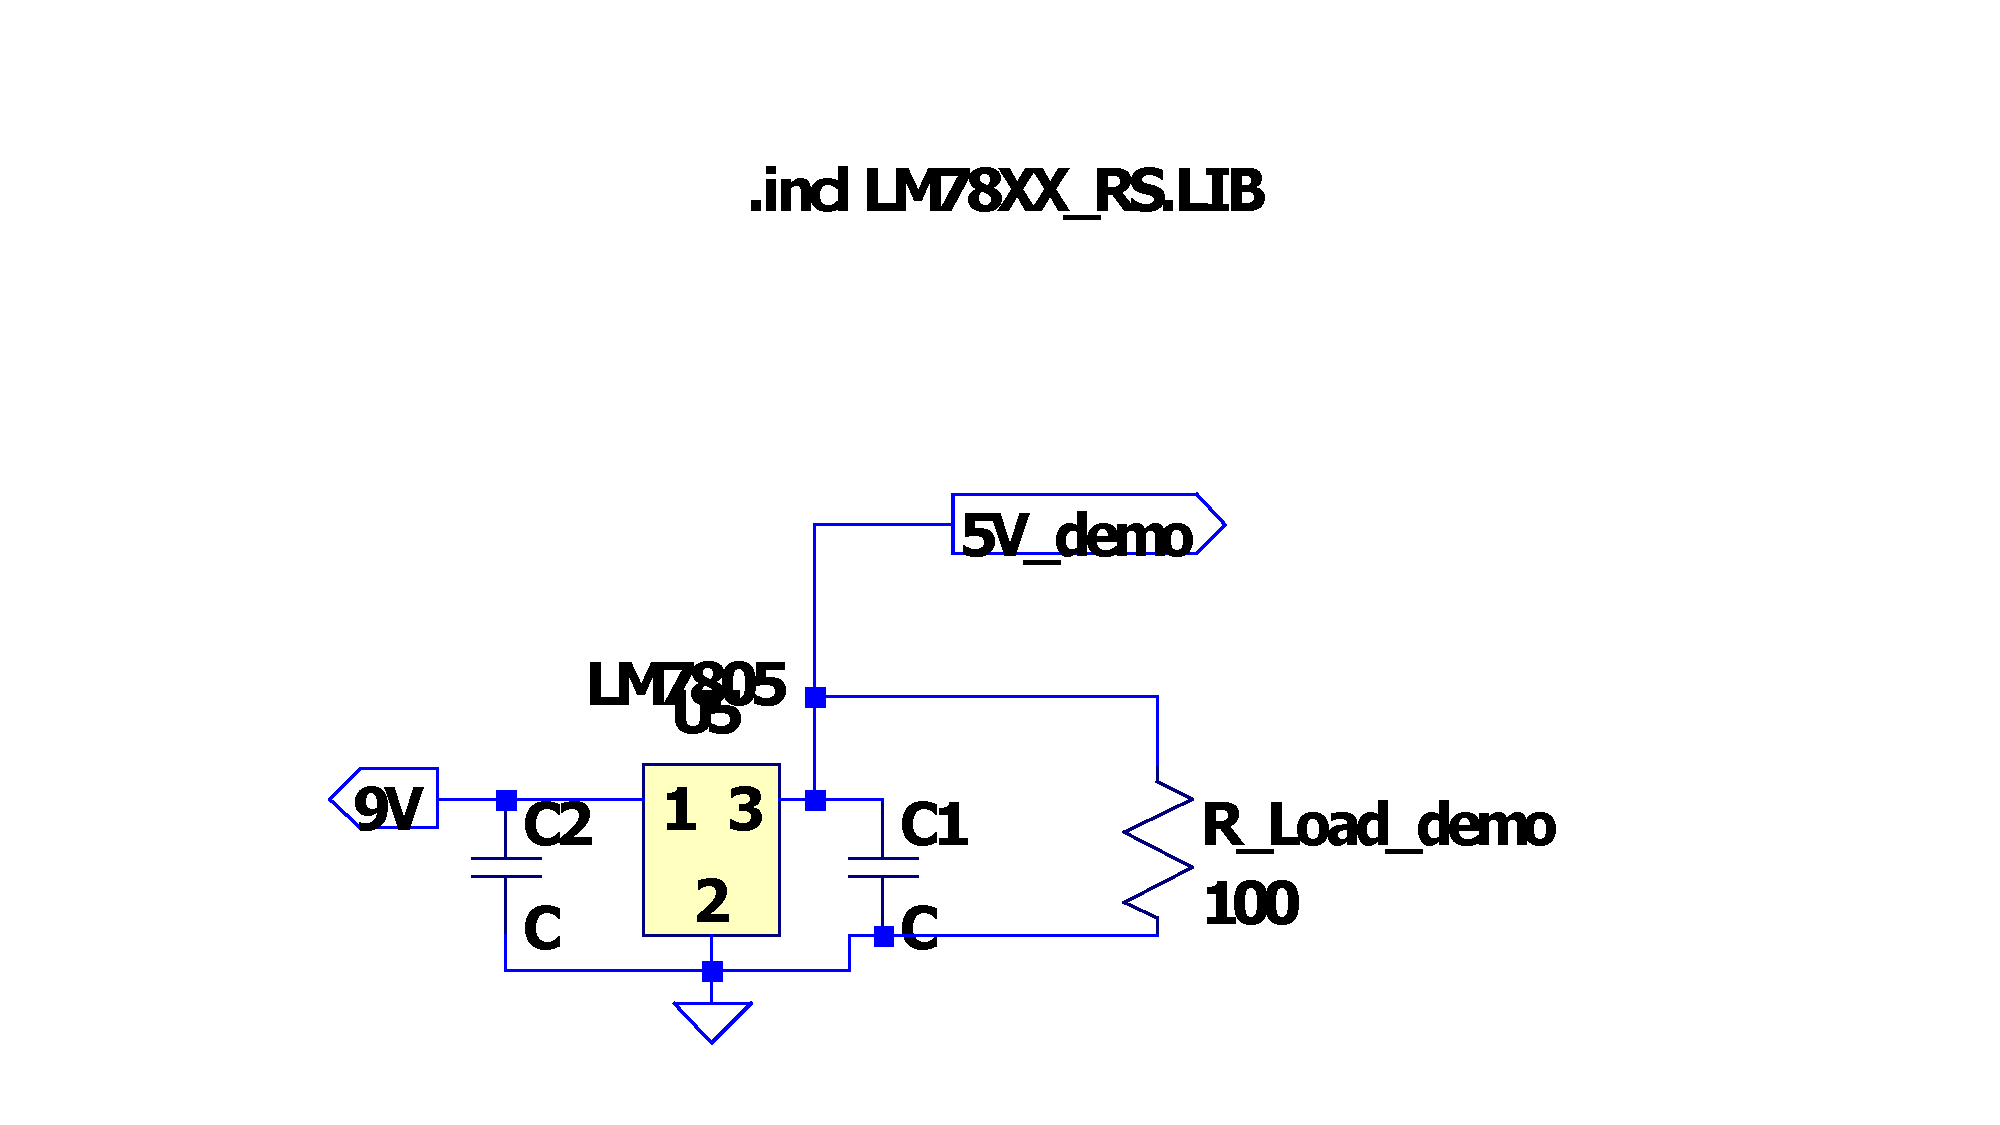
\includegraphics[width=\linewidth]{./Figures/E344_Ass1VoltRegulator_cct}
	  \caption{Linear voltage regulator.} \label{subfig:linear_circuit_diagram}	
   \end{subfigure}
   \begin{subfigure}[]{0.45\textwidth}
  	 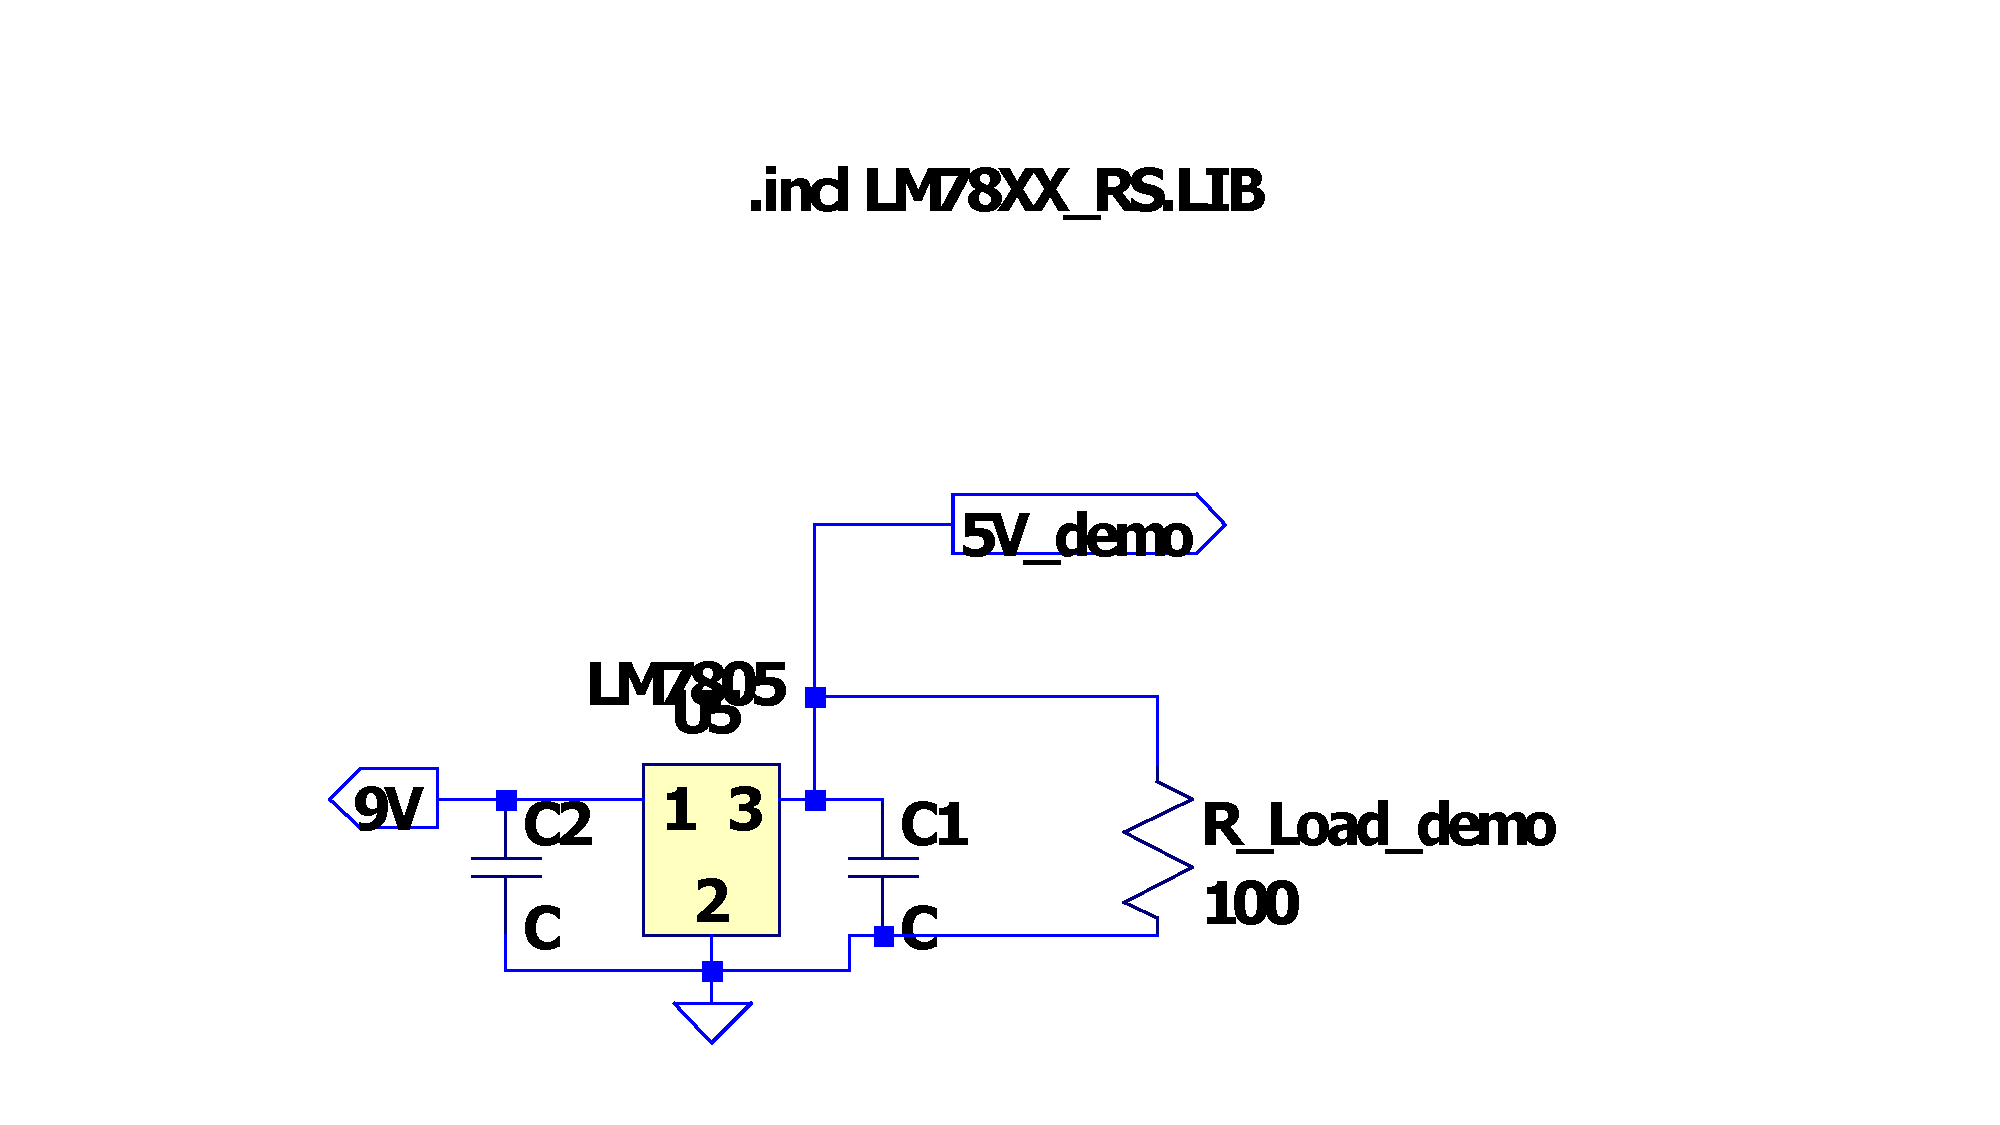
\includegraphics[width=\linewidth]{./Figures/E344_Ass1VoltRegulator_cct}
	  \caption{Switchmode voltage regulator.} \label{subfig:switchmode_circuit_diagram}	
   \end{subfigure}
   \begin{subfigure}[]{0.95\textwidth}
  	 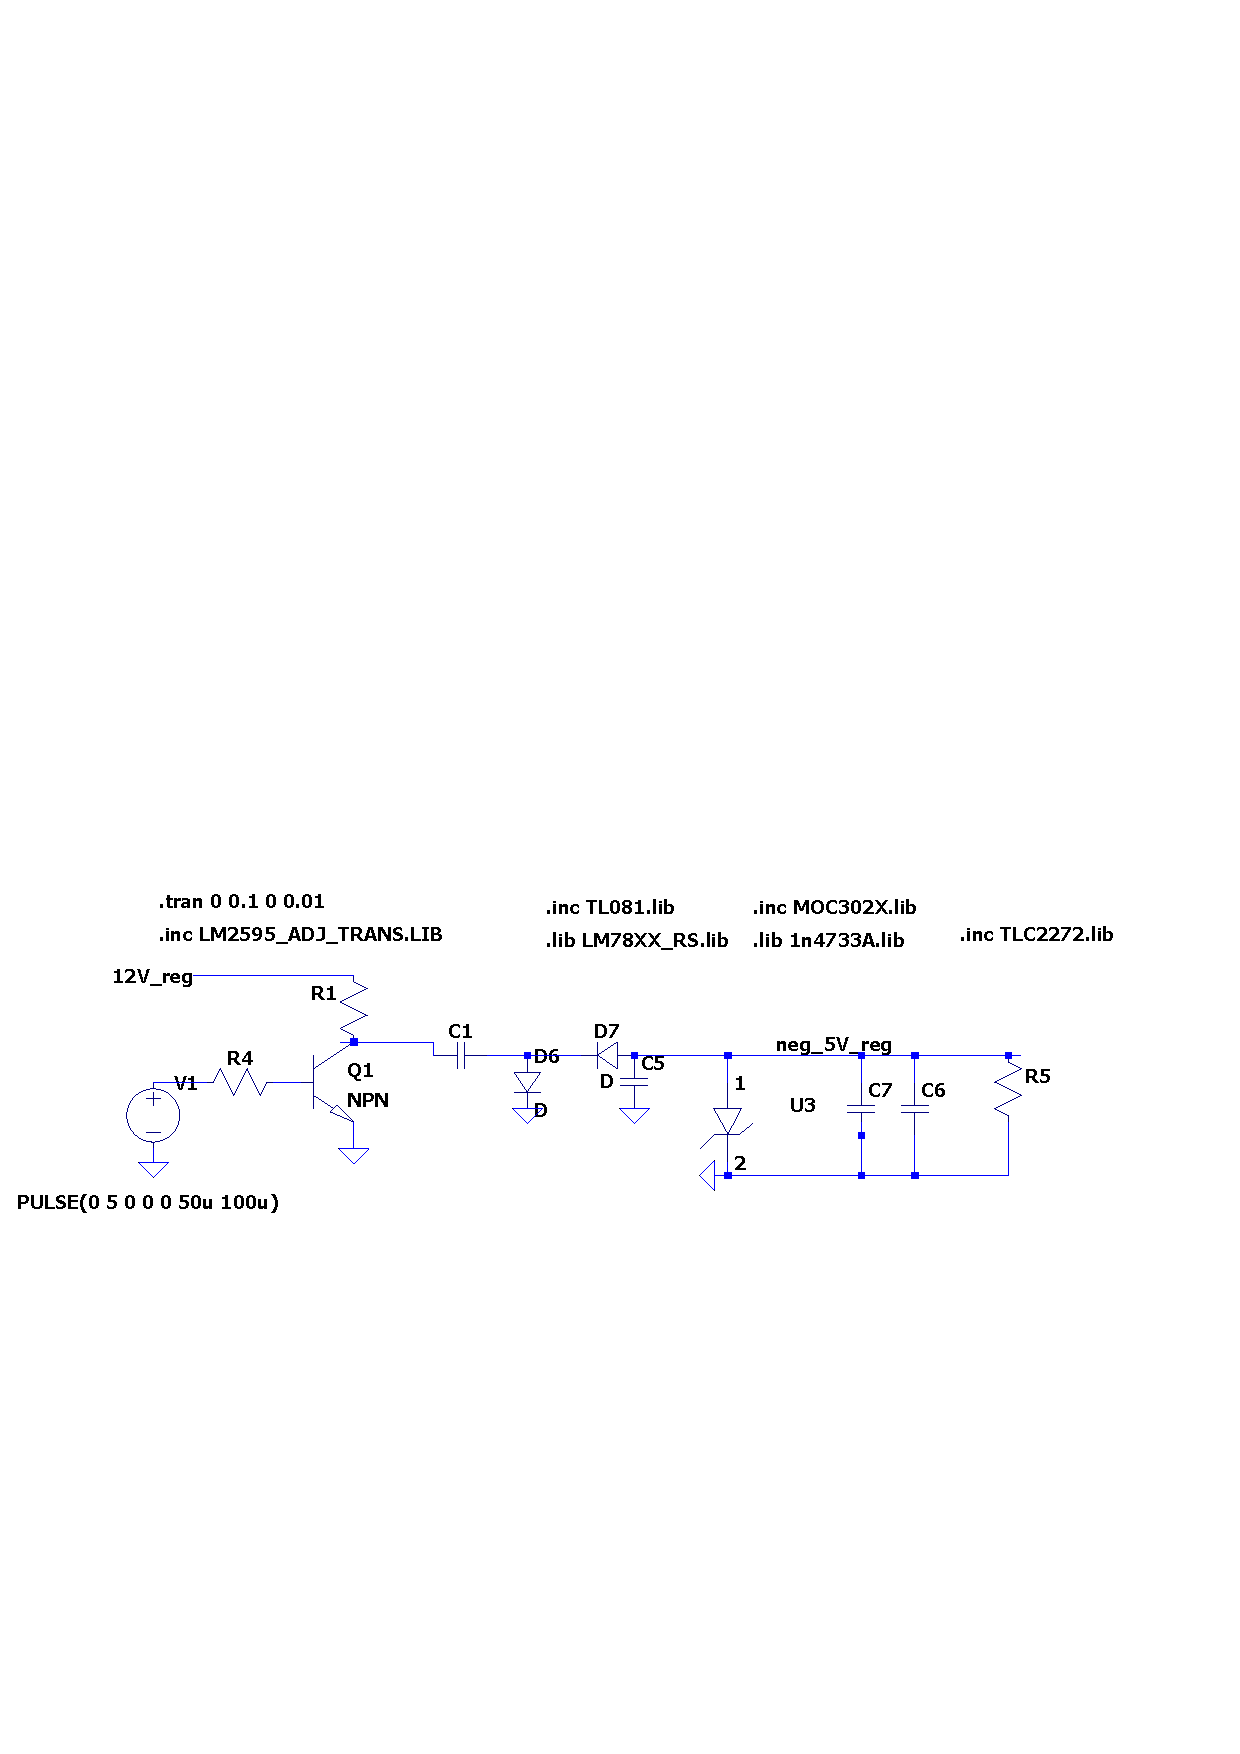
\includegraphics[width=\linewidth]{./Figures/CctDia}
	  \caption{Chargepump voltage regulator.} \label{subfig:chargepump_circuit_diagram}	
   \end{subfigure}
   
   \caption {Circuit diagrams of the two voltage regulators, and another irrelevant one}.

      \label{fig:circuit_diagram}
 \end{figure}
\section{Current sensor}\label{sec:current_sensor_design}

\vfill


